\documentclass[a4paper,12pt]{article}
\usepackage{fullpage}
\usepackage[british]{babel}
\usepackage[nodayofweek]{datetime}
\usepackage[none]{hyphenat} 
\usepackage{hyperref}
\usepackage{listings}
\usepackage{color}
\usepackage{float}
\usepackage[pdftex]{graphicx}
\usepackage{epstopdf}
\definecolor{lightgray}{rgb}{.9,.9,.9}
\definecolor{darkgray}{rgb}{.4,.4,.4}
\definecolor{purple}{rgb}{0.65, 0.12, 0.82}

\lstdefinelanguage{sdtl}{
  keywords={new, true, false, function, return, if, while, else, output, input},
  keywordstyle=\color{blue}\bfseries,
  ndkeywords={this},
  ndkeywordstyle=\color{darkgray}\bfseries,
  identifierstyle=\color{black},
  sensitive=false,
  comment=[l]{\#},
  commentstyle=\color{purple}\ttfamily,
}
\lstset{
   language=sdtl,
   backgroundcolor=\color{lightgray},
   extendedchars=true,
   basicstyle=\footnotesize\ttfamily,
   showstringspaces=false,
   showspaces=false,
   numbers=left,
   numberstyle=\footnotesize,
   numbersep=9pt,
   tabsize=2,
   breaklines=true,
   showtabs=false,
   captionpos=b
}
\begin{document}

\title{Inferring Class Structures of Duck-Typed Variables Through Static Code Analysis}
\author{In-Ho Yi\\
i.yi@student.unimelb.edu.au
}
\date{\today}
\maketitle
\section{Introduction}
Contemporary dynamic-typing languages such as Python and ECMAScript utilise `duck-typing' as a way of allowing users to define and use classes on-the-fly. By allowing a programmer to dynamically create properties of variables, these languages allow a programmer to rapidly prototype models.\\
The aim of the proposed project is to apply static code analysis to infer class structures from the use of duck-typed variables.\\


\subsection{The Challenge of Analysing Duck-Typing Programs}
In traditional OOP languages such as Java and C\#, the task of statically analysing class structure is almost trivial. Programmers define the types and hierarchies in advance, and the declarations themselves are readily understandable by machine. There are tools available for translating a design diagram such as UML to a code stub, and vice versa.\\
Duck-typing languages, on the other hand, does not include a finite definition of a class structure. Consider the following declaration of class in Python:\\
\begin{lstlisting}[caption=Python class creation, language=Python]
from random import random
class ExampleA:
    def __init__(self):
        self.someProperty = 'a'
        if(random() > 0.5):
            self.otherProperty = 'b'
    def someMethod(self, a):
        print(a)
a = ExampleA()
a.someMethod('Hello, world')
a.myProperty = 2
def newMethod(b):
    print(b)
a.newMethod = newMethod
a.newMethod('Hello, world')
\end{lstlisting}
There are several difficulties of statically analysing this code. First, declarations of members are dynamic, and the type itself can even depend on a control flow. In case of class ExampleA, instances have 50\% chance of having `otherProperty' as a member.\\
Second, after the initial creation of an instance, a programmer can liberally extend the class by declaring a new members dynamically.
\subsection{Examples of the Proposed Solution}
\subsubsection{Fruits}
Suppose we have the following code fragments written in a duck-typing language:\\
\begin{lstlisting}[caption=Example: Fruits]
function Fruit(name) {
	this.name = name;
}

function juiceMe() {
	# juicing me
}

apple = new Fruit('apple');
apple.juice = juiceMe;

grape = new Fruit('grape');
grape.juice = juiceMe;

banana = new Fruit('banana');

watermelon = new Fruit('watermelon');
\end{lstlisting}
If we construct a finite lattice $L = (2^P, \supseteq)$, P being the set of all known properties and methods of all instances of classes, we obtain the following lattice:\\
\begin{figure}[H]
	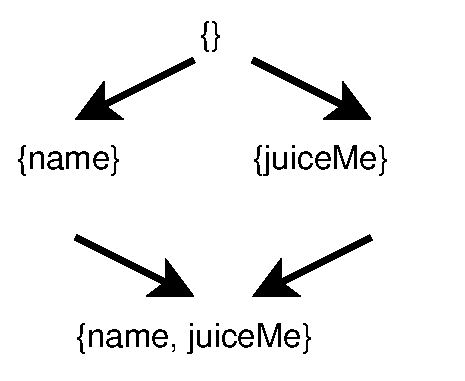
\includegraphics{lattice1.eps}
	\centering
	\caption{Lattice of all known properties and methods}
\end{figure}
We now construct a similar lattice $M = (2^V, \supseteq)$for all know variables in a program:\\
\begin{figure}[H]
	\includegraphics{lattice2.eps}
	\centering
	\caption{Lattice of all variables}
\end{figure}
If we map elements of $M$ to $L$, $N = L \mapsto M$, we have a lattice sufficient to represent the class types of all variables at any given point in runtime. Our ambition is to devise a fixed point iteration, which can be performed over normalised set of instructions, to map a particular element of the lattice to each point of control flow.\\
\begin{figure}[H]
	\includegraphics{lattice3.png}
	\centering
	\caption{Mapping of two lattices}
\end{figure}

\subsubsection{View Model Development in a Duck-Typing Language}
In Model-View-ViewModel(MVVM) development methodology, developers sketch out a view model first, bearing in mind possible structures of models and views. Suppose such developer writes a code in the following manner:\\
\begin{lstlisting}[caption=Controller written in a Duck-Typing language]
controller = new Controller();
controller.form = new Form();
controller.db = new Db();

function UpdateAge() {
	age = this.form.age;
	personId = this.form.personId;
	this.db.UpdateAge();
}
controller.PerformUpdateAge = UpdateAge;

function DisplayAge() {
	age = this.db.GetAge(this.form.personId);
	this.form.ShowAge(age);
}
controller.PerformDisplayAge = DisplayAge;

# Testing

controller.form.age = 20;
controller.form.personId = 110;
controller.PerformUpdateAge();
if(controller.db.GetAge(110) != 20) {
	output 1 # Test 1 failed
}
controller.PerformDisplayAge();
if(controller.form.shownAge != this.db.GetAge(110)) {
	output 2 # Test 2 failed
}
\end{lstlisting}

\section{Toy Language}
We will define a toy language that we name Simple Duck-Typing Language (SDTL). The design goal is to come up with a largely subset of ECMAScript expressive enough to cover the topic without losing generality of the argument. The language features dynamic declaration of functions, primitive variables (int, bool) and objects (through \textit{new} keyword), to which a programmer can dynamically assign variables or functions to their properties.\\
SDTL does not allow explicit class definition, as in Python, or prototyping, as in ECMAScript. However, it is argued here that class definitions and prototypes can be normalised as a series of dynamic declaration.\\

\subsection{Program}
In SDTL, as in other script languages, a program is a list of statements. Formally,\\
$P \rightarrow S$\\

\subsection{Statement}
In SDTL, statements are the essential elements of the program. First of all, a statement can be an empty string, making an empty input a valid program.\\\\
$S \rightarrow \epsilon$\\
Statement can also be a concatenation of statements.\\\\
$S \rightarrow S\  S$\\
Now we turn to non-trivial definitions. We define an assignment statement.\\\\
$S \rightarrow Lexpr = Expr$\\
Here we make a distinction between left expression($Lexpr$) and expression($Expr$). A left expression is an expression that is capable of designating a memory location, such as a symbol or a member of an object. Naturally, a left expression is a subset of an expression.\\\\
$S \rightarrow Expr$\\
Statement can also be an expression. An evaluated value, if there is one, will be discard. If a programmer chose to use this construct, the intention of his or hers would be to use a side-effect of an expression evaluation, e.g. calling a database function to generate a side-effect.\\\\
$S \rightarrow output\  Expr$\\
We define \textit{output} statement, with which a programmer can print out result of numeric evaluation to console. For the purpose of simplicity, we assume that only numeric expressions are printed.\\\\
$S \rightarrow if\ (Expr)\ {\ S\ }$\\
$S \rightarrow if\ (Expr)\ {\ S\ }\ else\ {\ S\ }$\\
We introduce \textit{if} statement here. If the $Expr$ evaluates to be a boolean TRUE, the first statement is executed, otherwise, else statement is executed (if given). Any $Expr$ that does not evaluate to be a boolean value will give rise to a runtime error.\\\\
$S \rightarrow while\ (Expr)\ {\ S\ }$
\textit{while} statement is also a standard one present in most C-like languages. If $Expr$ evaluates to be a boolean TRUE, it will execute $S$ and repeat from evaluating $Expr$ again. An $Expr$ that does not evaluate to be a boolean value will give rise to a runtime error.\\\\
$S \rightarrow F$\\
Now, an important feature of this language is that a function declaration is regarded as a statement. When function is declared, the signature and the body of the function is stored in a heap, and a symbol designating such function is stored in a symbol table. This symbol can be referred as an $id$ element, and hence a function name by itself becomes a registered symbol and can be referred as a valid $Lexpr$, allowing such ECMAScript-like code:\\
\medskip
\begin{lstlisting}[caption=Function declaration as a statement]
function theanswer()	{
	return 42;
}
universalanswer = theanswer;
output universalanswer();
\end{lstlisting}
The outout of such program is `42'.
\section{Static Analysis}
The analysis technique will generally be built up on the analysis of monotone framework. A powerset of a set of properties associated with a variable can be thought of as a finite Lattice. By performing dataflow analysis over such Lattice, we will be able to tell what properties are assigned to a variable.\\
\subsection{Single Variable Analysis}
A forward analysis of the assignment of properties will give what properties are declared at a given point, hence it will tell what kind of duck is at the point. A backward analysis of the use of properties will give an implied class structure of a variable.\\
\subsection{Multi-Variable Analysis}
Aforementioned analysis can be extended to multi-variable scenario, by creating a mapping from variables to the superset of all properties that are used in all variables.
\subsubsection{Class Relations}
By comparing the properties set of two different variables, we will be able to tell whether two variables are the same kind of ducks (if they share the exact same set of properties), or if one variable is a base class of another (if one sits up in the lattice). If they are siblings, we will be able to infer the base class structure by calculating the upper bound of two sets of properties in the lattice.
\subsubsection{Inheritance}
Given multiple variables, if we calculate an upper bound of list of properties that encompasses all variables will give a base class definition analogous to object class in Java language. A more useful result would be to calculate several upper elements that encompasses a sizeable number of elements. If a variable is under multiple upper elements, this relationship can be thought of as a multiple inheritance. Possible heuristics for deciding the granularity of such an analysis will be thought of and experimented with. Such a problem can be hard (hardness will be argued if necessary), and possible algorithmic approach will also be discussed.\\
Modern OOP languages such as Java introduced a concept of interface, so as to 
avoid multiple inheritance from classes. An upper element with a relatively 
fewer properties and large number of inheriting variables can be thought of 
as exhibiting an interface-like feature. We will devise a way to numericise 
such a feature to produce an index of interface-likeness. Such an analysis 
will help a programmer decide a proper class structure should they decide to 
move on to a more serious programming language from a rapid prototype.
\section{Conclusion}
Performing static code analysis on duck-typing programs will provide useful 
informations in the context of error-proofing and rapid prototyping. The 
result of such an analysis will be useful in two ways.\\ 
Firstly, it will allow IDEs to be able to guard against potential mistakes, 
by suggesting what kind of ducks certain parameters can be in a certain 
context. Thus, it will help prevent bugs resulting from mistyped names.\\
Secondly, it will allow RAD tools to suggest possible class definitions and 
their hierarchies by analysing the use of certain variables. The result of 
such an analysis will particularly be useful in the context of test-driven 
development paradigm.\\
\end{document}